% \begin{figure}[htpb]
%   \centering
%     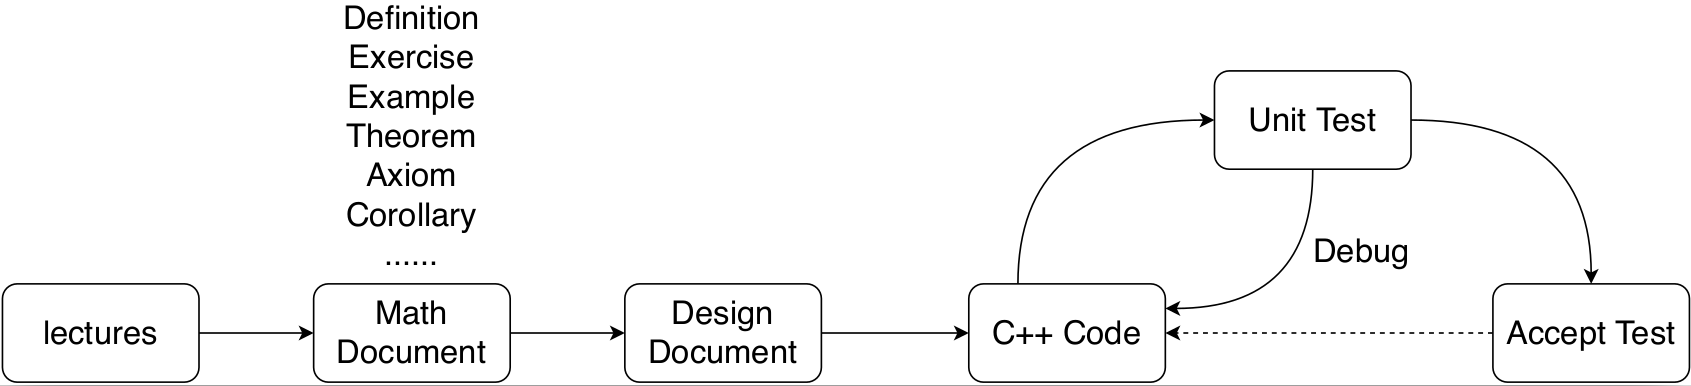
\includegraphics[width=0.4\textdwidth]{png/designPattern.png}
%   \caption{Design pattern}
%   \label{fig:designpattern}
% \end{figure}
\begin{center}
  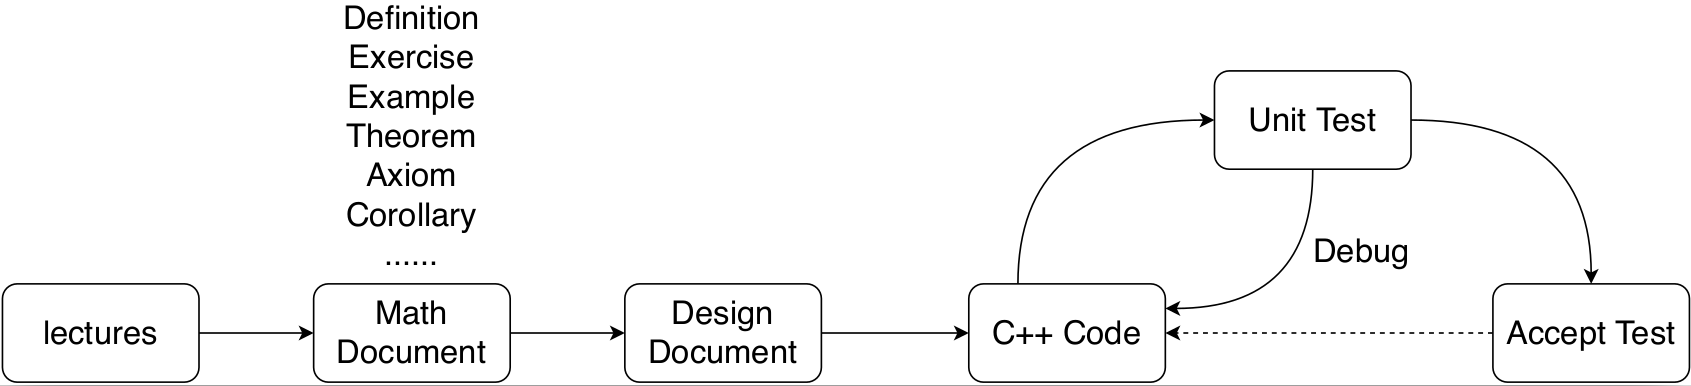
\includegraphics[width=0.45\textwidth]
     {png/designPattern.png}
\end{center}
\begin{thm}[The fundamental theorem of linear algebra]
  If $V$ is finite dimensional and $T\in {\cal L}(V,W),$
  then range $T$ is a finite-dimensional subspace of $W$
  and
  \begin{equation}
    \label{eq:1}
    \dim V= \dim {\cal N}( T)+ \dim {\cal R}(T).
  \end{equation}
\end{thm}

\begin{coro}
  For a matrix $A:\mathbb{R}^m\rightarrow\mathbb{R}^n$,
  \begin{align}
    \mathbb{R}^n&={\cal R}(A)\oplus {\cal N}(A^T),\label{eq:matrix}\\
    \mathbb{R}^m&={\cal R}(A^T)\oplus {\cal N}(A).
  \end{align}
  where ${\cal R}(A)\perp {\cal N}(A^T)$ and
  ${\cal R}(A^T)\perp {\cal N}(A)$.
\end{coro}

\begin{proof}
  For $\forall \mathbf{v}\in \{\mathbf{v}\in\mathbb{R}^m
  \vert A\mathbf{v}\in {\cal N}(A^T)\},$
  we have
  \begin{equation*}
    \grb{A\mathbf{v},\mathbf{v}}
    =\grb{\mathbf{v},A^T\mathbf{v}}=0,
  \end{equation*}
  which implies $\mathbf{v}=\mathbf{0}$.
  Thus ${\cal R}(A)\cap {\cal N}(A^T)=\{\mathbf{0}\}$
  and (\ref{eq:2}) follows from (\ref{eq:1}).
\end{proof}

%%% Local Variables:
%%% mode: latex
%%% TeX-master: "../notesNumericalSolution"
%%% End:
